%%%%%%%%%%%%%%%%%%%%% chapter.tex %%%%%%%%%%%%%%%%%%%%%%%%%%%%%%%%%
%
% sample chapter
%
% Use this file as a template for your own input.
%
%%%%%%%%%%%%%%%%%%%%%%%% Springer-Verlag %%%%%%%%%%%%%%%%%%%%%%%%%%
%\motto{Use the template \emph{chapter.tex} to style the various elements of your chapter content.}
\chapter{Scope and Structure of This Book}
\label{intro-whatthisbookisabout} % Always give a unique label
% use \chaptermark{}
% to alter or adjust the chapter heading in the running head

\chapter{What This Book Covers}

Active Directory Security: Attacks and Defenses
This book is a practical guide to attacking and defending Active Directory (AD) environments, using real-world techniques drawn from nearly 20 years of red team operations and adversarial emulation. The focus is on abusing built-in features and overlooked configurations - no exploits, no frameworks - just reliance on human-error that provides tried and true methods that work in the field.

Often, organizations that use Active Directory (AD) think that they are secure because of a strong vulnerability management program and patching new threats and vulnerabilities the minute they are released. Their vulnerability scans may come up clean week after week, but are they truly secure? If they are neglecting AD security, then most likely not.

I have performed penetration tests against many network infrastructures where I was unable to find any directly exploitable services or applications but was able to gain a toehold in Active Directory, take over the internal and DMZ domains, and issued 10+ high-risk findings related to AD in their final deliverable-the pentest report.

As an ethical hacker, ignoring AD typically results in leaving a massive attack surface on the table. It's practically akin to leaving the front door to your house open with a huge sign that reads "Please, Come In. Everyone!" At the same time, organizations that are neglecting to implement strong AD security infrastructure also open themselves up to a plethora of attacks.

\section{Learning Active Directory For Beginners}
Active Directory is a vast topic and can be overwhelming to grasp when first approaching it. My number one tip for anyone starting with AD is to first gain a thorough understanding of the fundamental key components that make up an Active Directory environment and how they interplay together.

Until you understand these key components and can recall from memory the most important ones to enumerate during a penetration test (users, groups, computers, Organizational Units (OUs), Access Control Lists (ACLs), Group Policy Objects (GPOs), local administrator access, to name a few), it will be challenging to follow along with forthcoming AD-related topics.

Below is a list of some key components I recommend learning about in-depth before diving deeper into AD and the key items to focus on whilst performing enumeration. If you are a beginner just starting out, I recommend taking a look at the "Introduction to Active Directory" module at HTB Academy. It will take you from zero knowledge of Active Directory to a decent, well-rounded understanding of its key fundamental components.

Once you have this core knowledge under your belt, you can move onto more advanced topics such as attacking and enumeration, exploitation and post-exploitation weaponization and delivery of attack payload(s0, and more. Learning as much as you can about AD alongside with this book will teach you the necessary fundamentals needed to navigate Windows domain-joined information systems from the command line using such tools like PowerShell, BloodHound, and PowerView.

\subsection{Key AD Component Terminology}
\textbf{Object:}
An object can be defined as ANY resource that is present within an Active Directory environment, such as OUs, printers, users, domain controllers, and so on.

\textbf{Attribute:}
Every object in Active Directory has an associated set of attributes that are used to define its characteristics. A computer object contains attributes such as the hostname and DNS name servers.

All attributes in AD have an associated LDAP name that can be used when performing LDAP queries, such as \texttt{displayName} for Full Name and given for First Name.

\textbf{Schema:}
The Active Directory schema is essentially the blueprint of any enterprise AD environment. It defines what types of objects can exist in the AD database (NTDS.dit) and their associated attributes. It lists definitions that correspond to AD objects and holds information about each corresponding object. For example, users in AD belong to the class "user," and computer objects to "computers."

Each object has its own information (some required to be set and other an optional choice) that are stored in Attributes. When an object is created from a class, this is called \textit{instantiation,} and an object created from a specific class is called an \textit{instance} of that class. For example, if we take a computer named RDS01, this computer object is an instance of the "computer" class in AD.

\textbf{Domain:}
A domain is a logical grouping of objects such as computers, users, OUs, and groups. We can think of each domain as a different city within a state or country. Domains can operate entirely independently of one another to be connected via trust relationships.

\begin{figure}
    \centering
    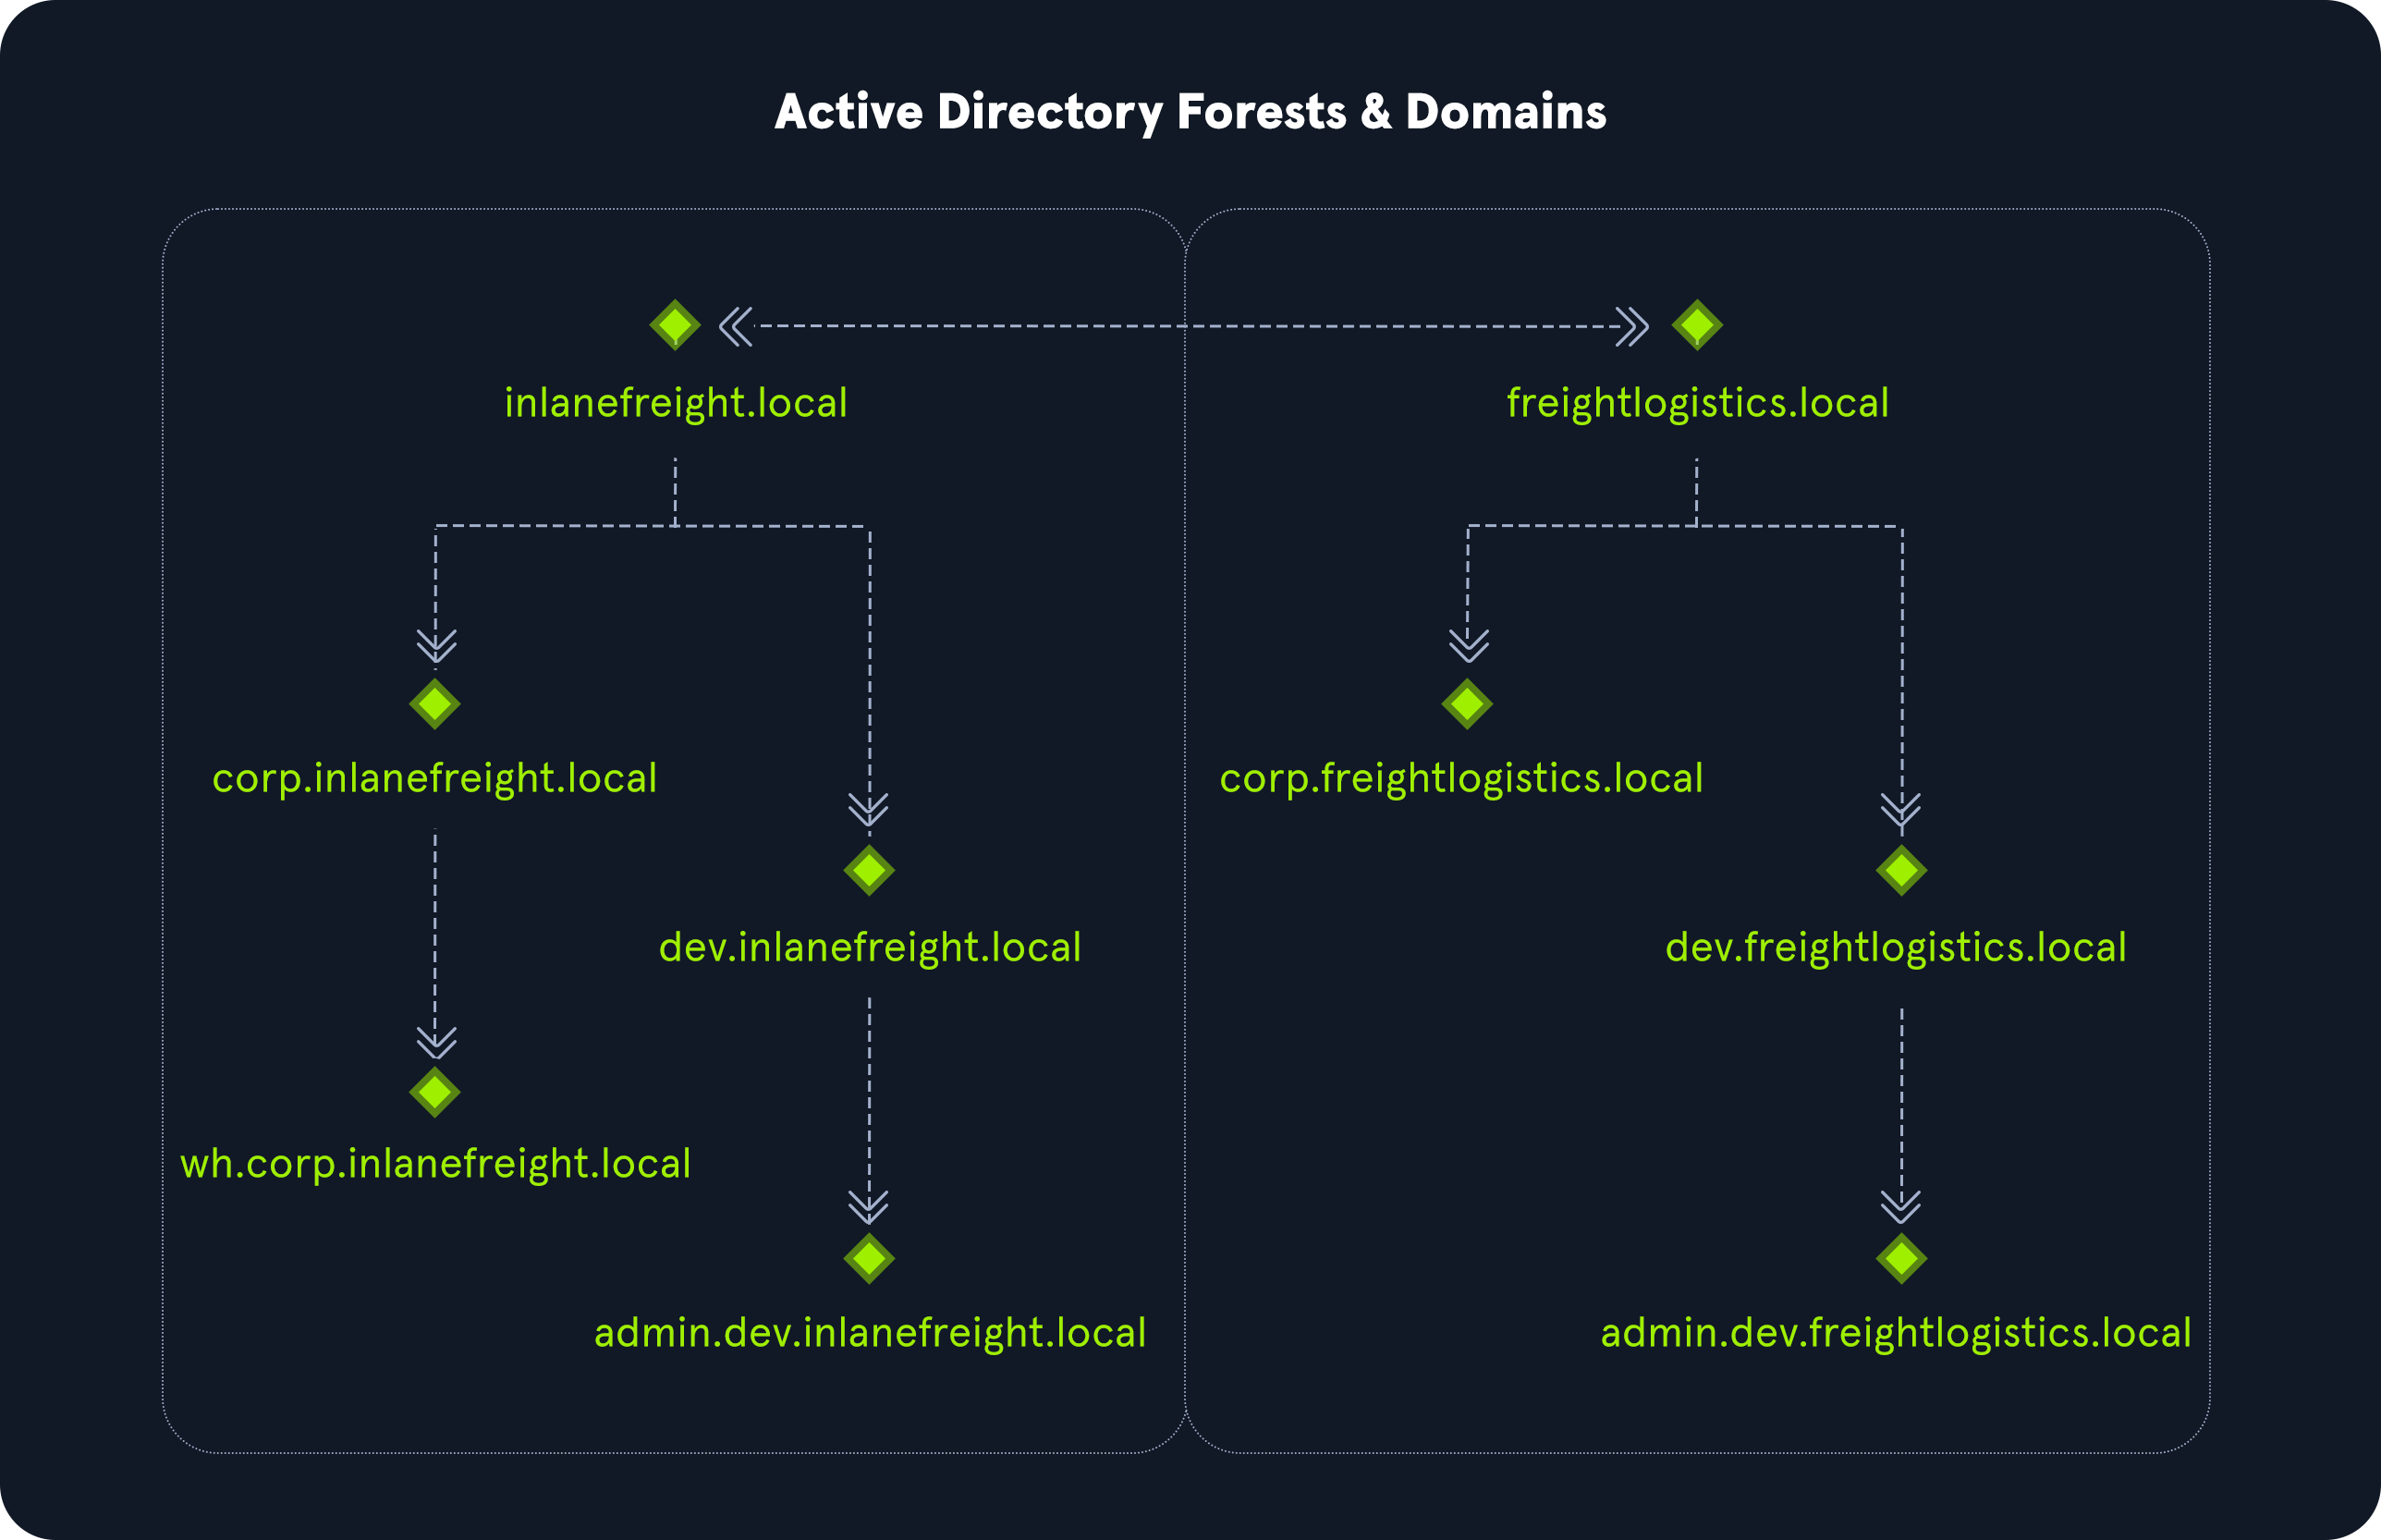
\includegraphics[width=0.75\linewidth]{domain.png}
    \caption{Domain Interconnections}
    \label{fig:placeholder}
\end{figure}


\textbf{Forest:}
A forest is a collection of Active Directory domains. It is the topmost container and contains all AD objects, including, but not limited to domains, users, groups, computers, and Group Policy Objects (GPOs). A forest can contain one or multiple domains and be thought of as a state in the U.S. or a country within the EU. Each forest operates independently but may have various trust relationships with other forests in the domain.

\textbf{Tree:}
A tree is a collection of Active Directory domains that begin at a single root domain. A forest is essentially a collection of AD trees and each domain within a tree shares a boundary with the other surrounding domains. A parent-child trust relationship is formed whenn a domain has been added under another domain in a tree. Two trees in the same forest cannot share a namespace.

Let us say we have two trees in an AD forest: inlanefreight.local and ilfreight.local. A child domain of the first would be corp.inlanefreight.local while a child domain of the second could be corp.ilfreight.local. All domains in a tree share a standard Global Catalog Service (GCS) which contains all information about objects that belong to the tree.

\begin{figure}
    \centering
    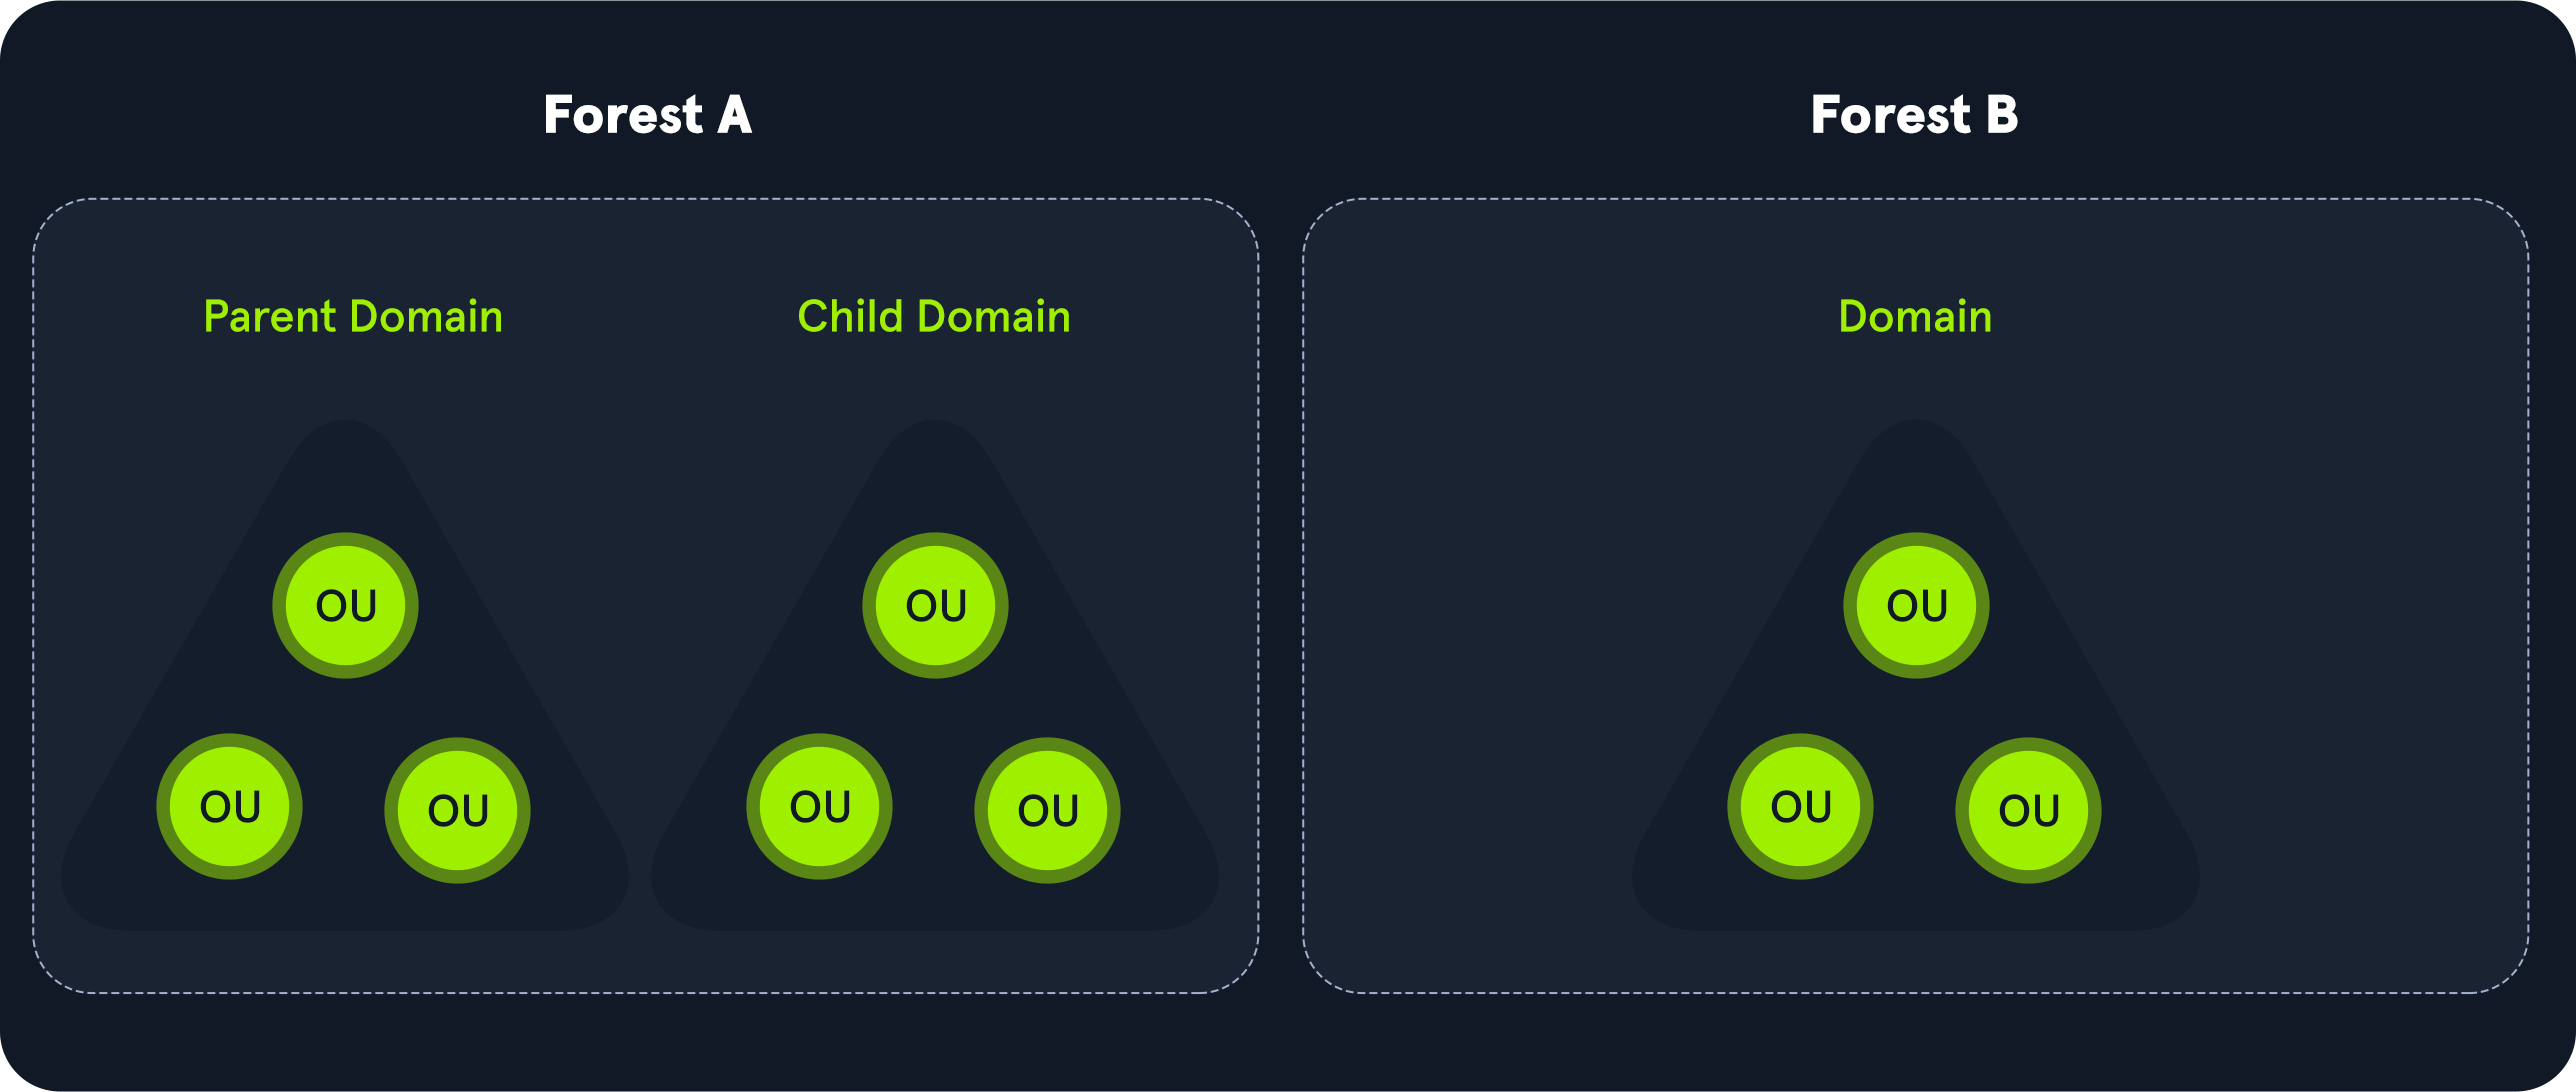
\includegraphics[width=0.75\linewidth]{domainstructure.png}
    \caption{Domain structure}
\end{figure}

\textbf{Container:}
Container objects hold other objects and have a defined place in the directory subtree hierarchical model.

\textbf{Leaf:}
Leaf objects do not contain other objects and are found at the end of the subtree hierarchy.

This book discusses the various aspects of Active Directory (AD) security, a critical component for managing user accounts and identities and for establishing trust and integrity through the use of restricted access management controls to resources in Windows Active Directory Server environments. This book covers attack vectors and vulnerabilities, such as privilege escalation through techniques such as Kerberoasting, Pass-the-Hash (PtH), and exploiting misconfigurations in services like Active Directory Certificate Services (AD CS) and Group Policy Objects (GPOs), emphasizing the role of tools like Mimikatz, PowerView, and BloodHound in these sophisticated cyberattacks. The book also highlights defensive strategies for defenders and blue teams, including implementing a tiered access model, least privilege, using Protected Administrative Workstations (PAWs) and Secured Administrative Workstations (SAWs), continuous monitoring for specific Windows Event Log IDs to pinpoint malicious activities, and the importance of patch management and regular penetration testing and security vulnerability assessments to secure the AD environment. Furthermore, the book goes into detail covering DNS-specific attacks like DNS Cache Poisoning and flooding, to showcase the importance and necessity of DNS security in protecting the overall AD network infrastructure.


\abstract{No more than 200 words.}

\section{Introduction to Active Directory Backdoors: Myth or Reality?}

Active Directory (AD) lies at the heart of most enterprise identity infrastructures, acting as the cornerstone of authentication, authorization, and policy enforcement across Windows-based networks. It manages users, computers, and services, governs access to shared resources on a network, and enforces organizational security policies across domains and enterprises. Because of its critical role in controlling who or what can access resources within an enterprise, AD represents a prime, juicy target for attackers. Compromising AD often equates to gaining control of the entire environment. From an attacker's view, it offers a single point of elevation. From a defender's viewpoint, it presents a complex and sprawling surface that is difficult to of your chapter content conformable to the Springer Nature layout.
\section{Context and Motivation}
In real-world enterprise AD environments, security teams - including systems administrators, incident responders, penetration testers, ethical hackers, and auditors - face a common challenge: ensuring the confidentiality, integrity, and availability of Active Directory in the face of growing complexity and increasingly advanced threat actors. AD is not only large, but also dynamic; users and permissions change constantly, and many of the risks lie in subtle or long-standing configurations rather than in 